%	JASA LaTeX Sample File, Preprint Sample
%
%  Beginner Latex users should refer to their favorite online documentation
%  here is one from the TeX Users Group 
%	https://www.tug.org/twg/mactex/tutorials/ltxprimer-1.0.pdf
%
%  Useful FAQ from  https://journals.aps.org/revtex/revtex-faq
% 

%%%%%%% For Preprint
%% For manuscript, 12pt, one column style

\documentclass[preprint]{JASA}
\usepackage[pdftex]{}
\graphicspath{{figures/}}
\usepackage[dvips]{epsfig,graphicx}
\DeclareGraphicsExtensions{.pdf,.jpeg,.png, .eps}
%%%%% Preprint Options %%%%%
%% The track changes option allows you to mark changes
%% and will produce a list of changes, their line number
%% and page number at the end of the article.
 %\documentclass[preprint,trackchanges]{JASA}


%% NumberedRefs is used for numbered bibliography and citations.
%% Default is Author-Year style.
% \documentclass[preprint,NumberedRefs]{JASA}

%%%%%%% For Reprint
%% For appearance of finished article; 2 columns, 10 pt fonts

% \documentclass[reprint]{JASA}

%%%%% Reprint Options %%%%%

%% For testing to see if author has exceeded page length request, use 12pt option
% \documentclass[reprint,12pt]{JASA}


%% NumberedRefs is used for numbered bibliography and citations.
%% Default is Author-Year style.
% \documentclass[reprint,NumberedRefs]{JASA}

%% TurnOnLineNumbers
%% Make lines be numbered in reprint style:
% \documentclass[reprint,TurnOnLineNumbers]{JASA}

%% Optional algorithm package. You can comment this out and
%% include another package if you prefer another way to make
%% algorithms examples (but please check that the package is compatible with 
%%Editorial Manager; see JASA-EL-TeXGuide.pdf).


\usepackage{algpseudocode}

\begin{document}

\title[JASA/Dynamic Grids for Finite-Difference Schemes]{Dynamic Grids for Finite-Difference Schemes: Changing Parameters of Musical Instrument Simulations in Real Time}
\author{Silvin Willemsen}
\email{sil@create.aau.dk}
\author{Stefania Serafin}
\affiliation{Multisensory Experience Lab, CREATE, Aalborg University, Copenhagen, Denmark}

\author{Michele Ducceschi}
\author{Stefan Bilbao}
\affiliation{Acoustics and Audio Group, University of Edinburgh, Edinburgh, Scotland}
 
% \author{Author Five}			
% \altaffiliation{Also at: Department, University, City, State ZipCode, Country.}
% \affiliation{Department3,  University3, City, State ZipCode, Country}


\preprint{Willemsen, JASA}		%  if you want want this message to appear in upper right corner of title page

\date{\today} 

\begin{abstract}
Simulating musical instruments using physical modelling is a well-established field. Among the reasons of why one would simulate an instrument rather than sample an existing one, is that one could extend the capabilities of this instrument beyond what is physically possible, such as changing material properties or size of the instrument on the fly. Many modelling techniques exist of which finite-difference time-domain (FDTD) methods are considered the most flexible and generalisable in terms of the type of systems they can model, both linear and nonlinear. These methods do, however, lack the capability of handling smooth parameter changes, something other techniques are better suited for. This article proposes a method to dynamically alter the grids of simulations based on FDTD methods by smoothly adding and subtracting points from the system. This allows for dynamic parameter changes in physical models of musical instruments which are based on this technique. Furthermore, this technique allows the stability condition that the schemes using FDTD methods are based on, to always be satisfied with equality and thus have the highest output bandwidth possible. 
\end{abstract}

%% pacs numbers not used

\maketitle

%  End of title page for Preprint option --------------------------------- %



\section{\label{sec:1} Introduction}
Simulation of musical instruments through physical modelling is a well established field...

% of simulating musical instruments rather than recording them and playing them back (samples), is the flexibility of control and playability of the instrument. Imagine trying to record the entire control space of a violin, i.e., all possible combinations of bowing force, bowing velocity and fingering positions. The recording procedure would take a great amount of time and resources, let alone the amount of data storage required to store all of the high-quality audio.

% Due to the vast parameter space of many instruments, using simulations is a much more viable solution for capturing the full expressivity of an instrument than sampling.


One of the incentives of simulating the physics of musical instruments rather than recording their real counterparts, is that we can manipulate the virtual instrument in physically impossible ways. Examples of this could be to change material properties, or even the shape of the instrument on the fly. An example of a real-world instrument that requires these manipulations is the trombone, where tube-length needs to be dynamic in order to play the instrument. In a companion article we describe a physical model of this instrument as a case study for the techniques presented here. 

Existing physical modelling techniques include mass-spring systems [REF] and digital waveguides [REF]. Modal synthesis [REF], though requiring some assumptions and simplifications for most systems, does allow for easy and smooth parameter changes and could thus be a good candidate for implementing the aforementioned manipulations. See for example [REF] and [REF]. Finite-difference time domain (FDTD) methods for physical modelling, though generally more computationally expensive than other techniques, are more flexible and generalisable and do not need as many simplifications as modal synthesis does. These methods subdivide continuous partial differential equations (PDEs) that describe the physics of the system at hand (string, tube, etc.) into a grid of discrete points in space and time. Below, a brief introduction about grids and their relationship to stability is explained.

\subsection{Grids and stability}
The grid spacing between two discrete points in space and the time step between two discrete moments in time are closely connected through a \textit{stability condition}. This condition dictates the maximum number of points allowed to describe system before it gets unstable and the simulation ``explodes''. The closer the number of points is to the stability condition, the higher the quality of the simulation. If the condition is satisfied with equality, the quality of the simulation is at a maximum. 
Furthermore, the stability condition depends on the parameters of the model, such as material properties or size of the system, i.e., parameters that could be changed on the fly.

It is possible to set and fix the number of points of a discrete system and tune the parameters away from the stability condition, ending up with a simulation with a lower quality (shown in the limited bandwidth of the output of the simulation) than could be.

This article proposes a method to smoothly add and subtract points from a system in real time so that the stability condition is always satisfied with equality. This allows for a simulation where the parameters can be changed on the fly without running into either stability or bandwidth issues. 

This article is structured as follows: 
\textit{NOTES:}
\begin{itemize}
\item Section 2: Background on PDE $\rightarrow$ FDTD $\rightarrow$ stability conditions 
\item Section 3: Dynamic grid
\item Section 4: Results
\item Section 5: Discussion
\item Section 6: Conclusions and Future work
\end{itemize}
\section{\label{sec:2} Introduction to FDTD Methods}
To aid the illustration of the proposed method, the 1D wave equation will be used. Consider a 1-dimensional system with length $L$ (in m) described by state variable $u = u(x, t)$ defined over space $x \in [0, L]$ and time $t \geq 0$. The partial differential equation (PDE) of the 1D wave equation is then described as
\begin{equation}\label{eq:1dwave}
    \frac{\partial^2 u}{\partial t^2}= c^2\frac{\partial^2 u}{\partial x^2}\ ,
\end{equation}
parameterised by wave speed $c$ (in m/s).
%continuous boundaries here?
This continuous system can then be discretised into points in space and time. The spatial variable can be discretised using $x_l = lh$ (read: $x$ at location $l$) with integer $l \in [0, \hdots, N]$, grid spacing (distance between two consecutive points) $h$ (in m) and total number of points $N + 1$ (including the boundaries) where $N$ is calculated as 
\begin{equation}\label{eq:numberOfPoints}
    N = \text{floor}(L/h).
\end{equation}
The temporal variable can be discretised using $t_n = nk$ with positive integer $n$, time step $k = 1/f_\text{s}$ (in s) and sample rate $f_\text{s}$ (in Hz). The state variable $u$ can then be approximated using $u(x,t) \approx u_l^n$, which can be read as: the state $u$ at spatial index $l$ and time index $n$.

The following operators can then be applied to $u$ to get the following approximations to the derivatives in Eq. \eqref{eq:1dwave}
\begin{subequations}\label{eq:operators}
    \begin{align}
         \frac{\partial^2u}{\partial t^2} \approx \delta_{tt}u_l^n &= \frac{1}{k^2}\left(u_l^{n+1}-2u_l^n + u_l^{n-1}\right)\label{eq:secondOrderTime}\\
         \frac{\partial^2u}{\partial x^2} \approx \delta_{xx}u_l^n &= \frac{1}{h^2}\left(u_{l+1}^n-2u_l^n + u_{l-1}^n\right)\label{eq:secondOrderSpace}
    \end{align}
\end{subequations}
Substituting these definitions into Eq. \eqref{eq:1dwave} yields the following finite-difference scheme (FDS)
\begin{equation}
    \delta_{tt}u_l^n = c^2 \delta_{xx}u_l^n
\end{equation}
Expanding the operators as in %the Eqs. in
\eqref{eq:operators} and solving for $u_l^{n+1}$ (which is the only unknown) yields the following update equation
\begin{equation}\label{eq:updateEq}
    u_l^{n+1} = 2u_l^n-u_l^{n-1} + \lambda^2 \left(u_{l+1}^n-2u_l^n + u_{l-1}^n\right).
\end{equation}
Here, $\lambda = ck/h$ is referred to as the Courant number and determines the quality and behaviour of the simulation. For stability, it can be shown -- using Von Neumann stability analysis [REF] -- that \begin{equation}\label{eq:CFL}
    \lambda \leq 1,
\end{equation}
referred to as the Courant-Friedrichs-Lewy (CFL) stability condition. The closer $\lambda$ is to this condition, the higher the quality of the output of the system (see Section \ref{sec:quality}) and if $\lambda = 1$ Eq. \eqref{eq:updateEq} provides an exact solution to Eq. \eqref{eq:1dwave}%(this is true for the 1D wave equation)
. One can rewrite Eq. \eqref{eq:CFL} in terms of grid spacing $h$ to get
\begin{equation}\label{eq:stabilityCond}
    h \geq ck,
\end{equation}
i.e., the grid spacing has a lower bound (for the discrete system to be stable), which is based on the sample rate and wave speed used. $N$ can then be calculated using Eq. \eqref{eq:numberOfPoints} with \eqref{eq:stabilityCond} written as an equality ($h = ck$) after which $h$ needs be recalculated based on $N$ (due to the flooring operation in Eq. \eqref{eq:numberOfPoints}) according to $h = L/N$. This causes the CFL condition in \eqref{eq:CFL} to not always be satisfied with equality. This results in a decrease in quality of the simulation described in the following section.

\subsection{Simulation Quality and Bandwidth}\label{sec:quality}
As mentioned before, the Courant number $\lambda$ decides the quality of the simulation. Choosing $\lambda < 1$ will decrease this quality in two ways. Firstly, it will decrease the maximum frequency that the simulation is able to produce, i.e., it will decrease the bandwidth of the system output. See Figure \ref{fig:bandWidths}.
%
\begin{figure*}
\figline{\fig{bandwidthLambda1}{.25\textwidth}{(A)}
\fig{bandwidthLambda0.9}{.25\textwidth}{(B)}
\fig{bandwidthLambda0.5}{.25\textwidth}{(C)}
\narrowcaption{.25\textwidth}{Output bandwidths of Eq. \eqref{eq:updateEq} with $N = 50$ and (A) $\lambda = 1$, (B) $\lambda = 0.9$ and (C) $\lambda = 0.5$ excited with a raised cosine with a width of 5 at center-location $N = 25$. 
\label{fig:bandWidths}}}
\end{figure*}
%
By analysing the scheme in Eq. \eqref{eq:updateEq}, it can be shown that the maximum frequency produced by the system can be calculated using [REF]
\begin{equation}
    f_\text{max} = \frac{f_\text{s}}{\pi} \sin^{-1}(\lambda),
\end{equation}
shown in Figure \ref{fig:bandWidthFormula}.
%
Note, that only a small deviation of $\lambda$ from condition \eqref{eq:CFL} already has a profound effect on the bandwidth of the output.

\begin{figure}
%% \reprintcolumnwidth is the same in preprint and reprint for
%% ease of use for authors:
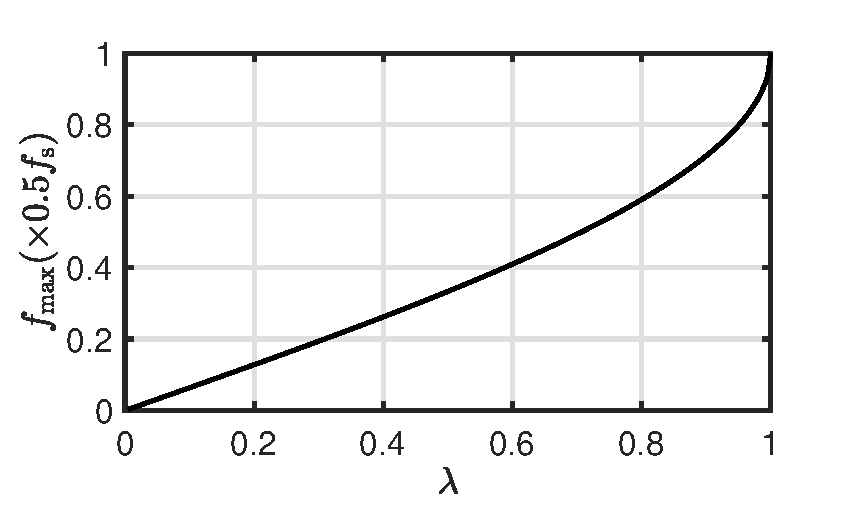
\includegraphics[width=\reprintcolumnwidth]{bandwidthPlot}
\caption{\label{fig:bandWidthFormula}{The effect of the Courant number $\lambda$ on the output bandwidth.}}
\end{figure} 

Secondly, choosing a value  numerical dispersion. This can be seen from Figure \ref{fig:bandWidths} where the harmonic partials get closer together at higher frequencies (i.e. get more inharmonic) as $\lambda$ decreases. This is an undesired effect.


Why would we want to be away from the condition
\subsection{Boundary Conditions}

As $x$ is only defined over a finite region, boundary conditions need to be given. Two possible conditions for Eq. \eqref{eq:1dwave} are
\begin{subequations}\label{eq:continuousBoundaries}
    \begin{align}
        u(0, t) = u(L, t) &= 0\quad \text{(Dirichlet)},\\
        \frac{\partial}{\partial x} u(0, t) = \frac{\partial}{\partial x} u(L, t) &= 0\quad \text{(Neumann)},
    \end{align}
\end{subequations}
or, `fixed' and `free' respectively. These conditions can be discretised as follows:
\begin{align}
    u_0^n = u_N^n &= 0 \quad\text{(Dirichlet)}\\
    \delta_{x\cdot} u_0^n = \delta_{x\cdot} u_N^n &= 0 \quad \text{(Neumann)}
\end{align}
where 
\begin{equation}
    \frac{\partial u}{\partial x} \approx \delta_{x\cdot}u_l^n = \frac{1}{2h}\left(u_{l+1}^n - u_{l-1}^n\right)
\end{equation}
is a second-order accurate approximation of the first-order spatial derivative.
\section{Dynamic Parameters}

\section{Dynamic Grids}

\bibliography{sampbib}
\end{document}




